\documentclass[12pt]{article}
\usepackage{times}
\usepackage{latexsym}
\usepackage{graphicx}
\usepackage{url}
\usepackage{float}
\usepackage[table,xcdraw]{xcolor}

\linespread{1}
\title{Anthropocentric Bias in Viral Genome Sequencing: Which Viruses Get Sequenced?}
\date{\today}
\author{Jacob Osborne}


\begin{document}

    \begin{titlepage}
        \begin{center}
            \vspace*{1in}
            \LARGE
            Anthropocentric Bias in Viral Genome Sequencing: Which Viruses Get Sequenced?

            \vspace*{1in}
            \large
            Completed for the Certificate in Scientific Computation \\
            Summer 2019

            \vspace*{1in}
            Jacob Osborne \\
            Computer Science \\
            Natural Sciences \\
            University of Texas at Austin

        \end{center}
        
        \vfill

        \noindent
        \rule{4in}{0.2mm} \\
        Dr. Claus Wilke \\
        Department Chair \\ 
        Integrative Biology \\

    \end{titlepage}


    %\begin{titlepage}
    %    \begin{center}
    %        \vspace*{1in}
    %        \LARGE
    %        Anthropocentric Bias in Viral Genome Sequencing: Which Viruses Get Sequenced?
    %
    %        \vspace*{1in}
    %        \large
    %        Jacob Osborne
    %
    %        \vfill
    %        [DEGREE PROGRAM] \\
    %        Dr. Claus Wilke, Integrative Biology \\
    %        \today
    %    \end{center}
    %\end{titlepage}
    
    \begin{abstract}
        The NCBI viral genomes database provides an extensive catalogue of genetic
        information from a variety of virus species. Yet, not all viruses are equal
        in their relevance to human life; there is some suspicion that those more
        directly important to our lives are significantly more likely to be
        sequenced than those that are not. To ascertain the existence and extent
        of this anthropocentric bias, a large-scale statistical analysis of the
        database was performed, and showed this was indeed the case.
        Specific patterns as to which viruses are more likely  to be sequenced
        are also documented and discussed.
    \end{abstract}

    \section{Introduction}

    The NCBI Viral Genomes database provides a large catalogue of viral genomes 
    sequenced by scientists around the world. It is the preeminent resource for
    obtaining records of viral genomes for scientific analysis.

    Yet, there is some doubt as to the extent to which the genomes catalogued
    therein can be taken as representative of viral genomes present in the
    natural world as a whole. We suspect the genomes of viruses that infect
    humans, domestic animals, and domestic plants - living things that are
    directly relevant to human life - are far more likely to be sequenced than
    the genomes of those which do not.

    The aim of this project, therefore, is to ascertain the extent of this
    anthropocentric bias in the NCBI database.

    \section{Data \& Methodology}
    
    \subsection{Overview}

    The NCBI viral genomes database does not provide information on the hosts
    of the viruses it contains records on. Thankfully, the Virus-Host Database provides
    linkages between the various NCBI databases' (including the Viral Genomes
    database) records for viruses and the records for their hosts. Therefore,
    this project uses data from the Viral-Host Database instead of the NCBI viral
    genomes database directly.

    The Virus-Host Database in its entirety - 14,042 unique records - is utilized in
    this project.

    This presents a difficulty, however - the Virus-Host Database's records are
    formatted as a relationship between a single virus and a single piece of
    literature that shows at least one host for that virus, with the hosts shown
    in that literature linked by the record, rather than as a relationship between a
    virus and its hosts.

    As such, the database was reformatted to a custom format, each entry providing
    a one-to-many relationship between a virus and its hosts.

    All data processing was performed via python script. Figures presented in the
    paper were generated using Matplotlib. A link to the github repository for this
    project is included in the appendix of this paper.

    \subsection{Preliminary Analysis}

    \begin{figure}[H]
        \begin{center}
            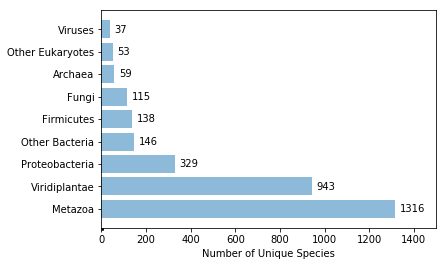
\includegraphics[width=100mm]{host_clades_figure.png}
            \caption{A breakdown of the kingdoms to which host species present in
            the database belong.}
            \label{host_clades_figure}
        \end{center}
    \end{figure}

    Figure \ref{host_clades_figure} shows the vast majority of host species in
    the database are either animals (Metazoa) or plants (Viridiplantae). Fungal
    host species are relatively uncommon in the data.

    \begin{figure}[H]
        \begin{center}
            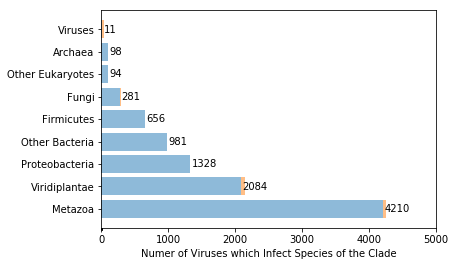
\includegraphics[width=100mm]{infects_clades_figure.png}
            \caption{A breakdown of viruses capable of infecting species of
            the given kingdom. The orange part represents viruses which can
            infect species of multiple kingdoms.}
            \label{infects_clades_figure}
        \end{center}
    \end{figure}

    

    We see a similar pattern in the number of virus species that find their
    hosts in a given clade, as shown in Figure \ref{infects_clades_figure}.
    The numbers there are roughly proportional to those in Figure
    \ref{host_clades_figure}, save that plants seem to make up a somewhat
    proportionately smaller portion of the data. It also shows that viruses
    which are capable of infecting species belonging to more than one distinct
    kingdom are extremely rare in the data set; thus, we can effectively ignore
    this overlap.

    These figures show a very small number of fungal species and fungal viruses
    present in the database. While there are a number of domesticated species of
    fungus, and a comparison involving these and their wild counterparts may
    prove useful to this investigation, this relatively small degree of data
    on the subject resulted in the decision to exclude fungal species and their
    viruses from the rest of the investigation, and focus solely on plants and
    animals.

    %\pagebreak

    \section{Results}
    
    \subsection{Distributions of Host and Virus Species}

    \begin{figure}[H]
        \begin{center}
            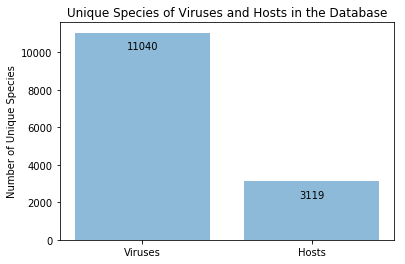
\includegraphics[width=100mm]{unique_species_figure.png}
            \caption{A comparison of the number of unique species of virus and of
            host present in the database.}
            \label{unique_species_figure}
        \end{center}
    \end{figure}

    As shown in Figure \ref{unique_species_figure}, there are just under 3
    times as many unique species of virus as of host. This means we can expect,
    for each host species in the database, multiple species of virus that infect
    it.

    This is not entirely the case, however. An examination of the distribution of
    the data, shown in Figure \ref{viruses_per_host_figure}, shows an enormous skew
    towards the lower end in the number of viruses per host species. In particular,
    well over half of the host species in the database - 1,797 species, to be exact -
    have only a single documented virus in the database.
    
    \begin{figure}[H]
        \begin{center}
            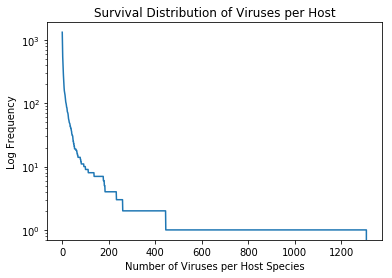
\includegraphics[width=90mm]{viruses_per_host_figure.png}
            \caption{The distribution of the number of unique species of virus
            capable of infecting each host species included in the database.}
            \label {viruses_per_host_figure}
        \end{center}
    \end{figure}

    Notably, a version of this graph using log scales for both axes - as shown in
    Figure \ref{log_viruses_per_host_figure} - shows a nearly straight line,
    indicating a simple exponential distribution is at play here.

    \begin{figure}[H]
        \begin{center}
            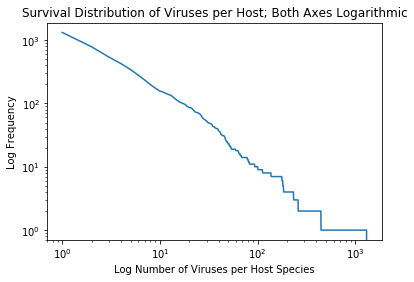
\includegraphics[width=90mm]{log_viruses_per_host_figure.png}
            \caption{Figure \ref{viruses_per_host_figure} with both axes on a
            logarithmic scale}
            \label{log_viruses_per_host_figure}
        \end{center}
    \end{figure}

    \begin{table}[H]
        \begin{center}
            \begin{tabular}{|l||c|}
                \hline
                Host species                                 & \# of Viruses \\ \hline\hline
                \textit{Homo sapiens}                        & 1,309         \\ \hline
                \textit{Mycolicibacterium smegmatis MC2 155} & 446           \\ \hline
                \textit{Solanum Lycopersicum} (Tomato)       & 261           \\ \hline
                \textit{Mycolicibacterium smegmatis}         & 234           \\ \hline
                \textit{Escheria coli}                       & 185           \\ \hline
                \textit{Bos taurus} (Cattle)                 & 182           \\ \hline
                \textit{Sus scrofa} (Pig)                    & 178           \\ \hline
                \textit{Mus musculus} (House mouse)          & 138           \\ \hline
                \textit{Pseudomonas aeruginosa}              & 113           \\ \hline
                \textit{Staphylococcus aureus}               & 101           \\ \hline    
            \end{tabular}
            \caption{The ten most common host species in the database.}
            \label{most_common_hosts_table}
        \end{center}
    \end{table}

    Species with the largest numbers of viruses seem to be a mix of domesticated
    species (both plants and animals) and an assortment of common bacteria.

    Unsurprisingly, the host species with by far the largest number of
    sequenced viruses - 1,309 distinct species - is \emph{Homo sapiens}, As
    shown by Table \ref{most_common_hosts_table}. However, the next most
    common hosts are rather surprising: two strains of 
    \emph{Mycolicibacterium smegmatis} - MC2 115 and one left unlabeled - with a
    combined 680 unique species of virus preying on them.

    \subsection{Wild and Domestic Host Species}

    \begin{figure}[H]
        \begin{center}
            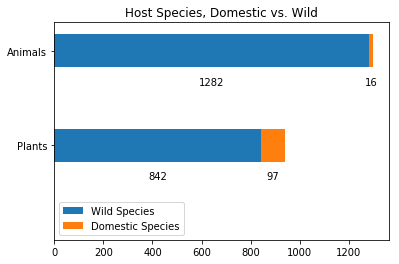
\includegraphics[width=100mm]{host_species_domestic_wild_figure.png}
            \caption{A comparison of the number of host species in the database
            that are domestic vs. those that are wild.}
            \label{host_species_domestic_wild_figure}
        \end{center}
    \end{figure}

    As shown in Figure \ref{host_species_domestic_wild_figure}, a quite small
    number of the plant and animal species appearing in the database are
    domesticated, vs. those that are wild. This is to be expected, as,
    ultimately, domesticated species make up a tiny portion of the species
    on Earth. These numbers, however, actually represent a much larger
    proprotion of the database than we would see if every animal on Earth
    were included in it.

    Notably, the proportion of plant species in the database which are
    domesticated is much larger than the proportion of animal species which
    are.

    \begin{figure}[H]
        \begin{center}
            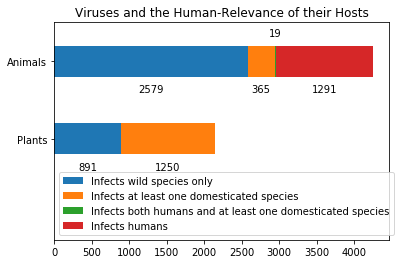
\includegraphics[width=100mm]{viruses_human_relevance.png}
            \caption{A comparison of which hosts viruses in the database
            infect, and whether their hosts are human-relevant (i.e. infect
            humans or a domesticated species)}
            \label{viruses_human_relevance_figure}
        \end{center}
    \end{figure}

    Figure \ref{viruses_human_relevance_figure} shows "Human-relevant" viruses
    - those that infect humans or species we have domesticated - make up more
    than half of the plant viruses in the database, and nearly half of the animal
    viruses.
    
    This appears grossly out of proportion to the relative numbers of domesticated
    and wild host species in the database. We can confirm this with a chi-squared
    test, setting up our categories as in Table \ref{domestic_wild_chi_test}, and
    with the null hypothesis "Whether or not a species is domesticated is independent
    of how many viruses that infect are sequenced."

    \begin{table}[H]
        \begin{center}
            \begin{tabular}{|c|c|c|c|}
                \hline
                                 & \textbf{Human-Relevant} & \textbf{Wild} & \textbf{Total} \\ \hline
                \textbf{Viruses} & 2,906                   & 3,470         & 6,376          \\ \hline
                \textbf{Hosts}   & 114                     & 2,124         & 2,238          \\ \hline
                \textbf{Total}   & 3020                    & 5594          & 8614           \\ \hline
            \end{tabular}
        \end{center}
        \caption{Categories for our chi test.}
        \label{domestic_wild_chi_test}
    \end{table}

    The test on this data gives us $\chi^2 = 1192.4394$, and therefore $p < 0.01$,
    rejecting the null hypothesis and showing our determination that these proportions
    don't match up is correct.

    It is also apparent that the number of viruses in each category is differently
    proportioned between plants and animals - with animals a proportionately
    larger number of animals are wild, versus those that are human-relevant.

    We can test this observation with another chi-squared test, this time using
    categories as in Table \ref{plants_animals_chi_test}, and with the null
    hypothesis "The number of human-relevant vs. wild viruses is independent of
    the number of plant vs. animal viruses."

    \begin{table}[H]
        \begin{center}
            \begin{tabular}{|c|c|c|c|}
                \hline
                                        & \textbf{Human-Relevant} & \textbf{Wild} & \textbf{Total} \\ \hline
                \textbf{Animal Viruses} & 1,656                   & 2,579         & 4,235          \\ \hline
                \textbf{Plant Viruses}  & 1,250                   & 891           & 2,141          \\ \hline
                \textbf{Total}          & 2,906                   & 3,470         & 6,376          \\ \hline
            \end{tabular}
        \end{center}
        \caption{Categories for the second chi test.}
        \label{plants_animals_chi_test}
    \end{table}

    The test on this data gives us $\chi^2 = 213.1386$, and thus $p < 0.01$,
    confirming that the two are not independent, and that plant viruses in the
    database are more likely to be "human-relevant" than animal viruses.
        
    \section{Discussion}

    \subsection{Bacteria \& their phages}

    On the subject of the most common host species in the database, as shown in
    Table \ref{most_common_hosts_table}, the results vis-à-vis eukaryotic species
    appearing in the table seem consistent with the overall results - humans are
    the most common host species, with the others being domesticated plants
    (tomatos) or domesticated animals (cattle, pigs, house mice). The bacterial
    species appearing in the table seem to be less intuitive, however.

    The reason for the predominance of \emph{Escheria coli}, \emph{Pseudomonas
    aeruginosa}, and \emph{Staphylococcus aureus}, however, seems clear with
    a bit of further investigation: \emph{Escheria coli} is commonly responsible
    for food poisoning, as well as being used as a model organism for bacteria
    in general; \emph{Pseudomonas aeruginosa} is an opportunistic pathogen, and
    infections involving it can be responsible for a variety of life-threatening
    conditions, including pneumonia and a variety of septic conditions \cite{pseudomonas};
    \emph{Staphylococcus aureus}, another opportunistic pathogen, is responsible
    for a variety of skin and respiratory conditions which can be life-threatening
    \cite{staph}.

    In short, all three are medically-significant pathogens.

    The predominance of \emph{Mycolicibacterium smegmatis} is more curious, as the
    bacterial species is not of any especial relevance. However, an examination of 
    its entries in the database reveals a possible reason why - nearly every virus
    attributed to it in the database is listed as being a phage of Mycobacteria in
    general. Futher, outside research reveals it was the first species of
    Mycobacteria for which a phage was discovered \cite{first_myco}.
    The Mycobacterium clade includes numerous species of pathogenic
    bacteria, including those responsible for tuberculosis and leprosy \cite{myco}. As 
    phage therapy has been a major focus in research for treatments for these
    diseases in recent years \cite{myco_phage}, it therefore becomes clear that
    \emph{Mycolicibacterium smegmatis}'s predominance in the database is a result
    of its use as a model organism for Mycobacterium phage research.

    The apparent predominance of pathogenic bacteria in the database appears
    to contradict the initial hypothesis of this investigation, but only in its
    most exact form. Pathogenic bacteria are extremely significant to human life,
    although in a different manner than domesticated plants and animals,
    so that virological research would also find itself biased towards them is in
    line with the contention that research into viral genomics is biased in an
    anthropocentric direction.

    The usage of the use of model organisms such as \emph{M. smegmatis} in phage
    research, however, presents a complication - it would require extensive manual
    curation to determine exactly which non-pathogenic bacteria in the database
    are serving as models for pathogenic species, versus which are being researched
    on their own merits. Such a determination would need to be made to perform any
    sort of detailed statistical analysis on this phenomenon.

    This places a deeper analysis of such outside the scope of this investigation,
    thus, is the reason why the rest of the results did not attempt to investigate
    this further, and why the remainder of this discussion will focus solely on
    plants and animals.

    \subsection{Viruses with domesticated or wild hosts}

    As shown in the first of the two chi-squared tests, outlined in Table
    \ref{domestic_wild_chi_test}, the database does, indeed, include a wildly
    disproportionately larger number of viruses for domesticated species and
    humans than it does for wild ones. It is extremely unlikely that this could
    be explained by domesticated species simply having more viruses than wild
    ones - even if we assumed they did, the discrepancy couldn't possibly be
    large enough to account for that we observe in the database. This suggests
    the confirmation of the existence of a significant anthropocentric bias
    in the database, as was initially hypothesized.

    The significance of this point to research into viral genomics as a whole is
    that the viral genomes in the database are not necessarily representative of
    the totality of viral genomics, so conclusions drawn from studies of the full
    collection of these genomes must, at the very least, be taken with a grain of
    salt.

    \subsection{Differences between plant and animal viruses in the database}

    Perhaps more interesting than the confirmation of the initial hypothesis,
    however, is that the \emph{degree} to which viral genome sequencing is slanted in
    an anthropocentric direction seems to vary depending on whether we are
    talking about plant or animal viruses, as shown in the second chi-squared
    test, outlined in Table \ref{plants_animals_chi_test}.

    In particular, the proportion of sequenced virus species which infect 
    "human-relevant" hosts is dramatically larger for those viruses which infect
    plants than those which infect animals. This cannot be explained by the
    exceptional presence of humans in the animal category, as removing
    human viruses from the data set would actually only reinforce this trend
    - to such an extent, in fact, that despite there being dramatically more
    animal viruses in the data base than plant viruses, the number of plant
    viruses which infect domesticated species would more than triple the number
    of animal viruses that infect domesticated species.

    One possible explanation for this would be that there is less interest or
    ability in the study the viruses of wild plants than there is in the study
    of viruses of wild animals, but this would fail to explain why viruses
    of domesticated plants also outnumber viruses of domesticated animals in a
    purely numeric, rather than only proportional manner - 1,250 viruses of
    domesticated plants are present in the database, versus 365 viruses of
    domesticated animals. While this may present \emph{part} of the reason
    why - there are, indeed, less viruses of wild plant species in the database
    than viruses of wild animal species - it cannot be the sole reason why.

    It is, instead, my hypothesis that the reason for this discrepancy is that
    disease is more relevant to the cultivation of crops than to raising
    domesticated animals. Livestock populations are typically relatively
    isolated from each other, with the stock belonging to a particular
    farmstead rarely interacting with that of others. By comparison, crop fields
    are often grown side by side, with the crops on the edge of one being in
    constant proximity to those in a neighbor's. This is little more than
    speculation, however - proper quantitative data on the economic impacts of
    crop viruses, and that of livestock viruses, would be necessary to make
    a definitive conclusion, and I was unable to find any such data for use
    in this research.

    \section{Acknowledgements}

    I thank Dr. Claus Wilke for supervising this project.

    \begin{thebibliography}{}

        \bibitem{pseudomonas}
        “\emph{Pseudomonas aeruginosa} in Healthcare Settings” cdc.gov, Centers for Disease Control and Prevention, 2 Apr. 2013.
        
        \bibitem{staph}
        “\emph{Staphylococcus aureus} in Healthcare Settings" cdc.gov, Centers for Disease Control and Prevention, 17 Jan. 2011.

        \bibitem{myco}
        “Mycobacterial Infections" MedlinePlus, U.S. National Library of Medicine, 7 Feb. 2019.

        \bibitem{first_myco}
        Gardner, Grace M., and Russell S. Weiser. “A Bacteriophage for Mycobacterium Smegmatis.” Proceedings of the Society for Experimental Biology and Medicine, vol. 66, no. 1, Oct. 1947, pp. 205–206, doi:10.3181/00379727-66-16037.
        
        \bibitem{myco_phage}
        Hatfull, Graham F. “Mycobacteriophages.” Microbiology spectrum vol. 6,5 (2018): 10.1128/microbiolspec.GPP3-0026-2018. doi:10.1128/microbiolspec.GPP3-0026-2018

    \end{thebibliography}

    \appendix

    \section{Project Code Repository}
    https://github.com/sable-cat/anthropocentric-sequencing

    \pagebreak

    \section{Reflection}

    Before starting this project, I'd already used the NCBI databases extensively
    in a number of my classes, so I didn't learn that much about them, ultimately.
    I did learn about the existence of the Virus-Host Database, and how to use it,
    however - as should be clear from the rest of my project, it proved immensely
    useful. I was thinking I'd have to manually curate host connections for a
    selection of viruses in the database, and that database saved me from that.

    I had to learn to use Matplotlib to generate figures/plots. Previously, I'd
    used a library in R to generate figures, but I made the decision to do all
    the code for this project in python, and thus was forced to teach myself
    Matplotlib. I do prefer it to any other such library I've used in the past -
    it's not exactly easy to use, but it provides a whole lot of control (just
    look at the little numbers I added to the bar graphs showing the exact
    size of each bar).

    This was also my first time doing statistical research and analysis without
    significant direction by a professor, as in my classwork. This is not to say
    Dr. Wilke contributed little to the project - that's certainly not the case -
    but that in class projects I had been given rather tight directions as to what
    the project should be about, how the final paper should look, etcetera, and
    this was the first time I was, essentially, free of that. It required far more
    creativity, and there were a number of times something didn't work out how I
    expected and I was rather lost on what, exactly, to do. At the same time, there
    were a number times where I was pleasantly surprised by a very interesting
    result (I was particularly elated when I first noticed the clear discrepancy
    between plant and animal viruses that the discussion spends so long elaborating
    on).




\end{document}